\documentclass[12pt]{article}%

\usepackage{fancyhdr}
\pagestyle{fancy}
\fancyhf{}
\fancyhead[R]{\thepage}

\usepackage{cmap}				
\usepackage{mathtext} 
\usepackage{listings}

\usepackage{biblatex}
\addbibresource{lib.bib}

\usepackage{euscript}
\usepackage{mathrsfs}

\usepackage[T2A]{fontenc}
\usepackage[utf8]{inputenc}
\usepackage[english,russian]{babel}
\usepackage{amsmath,amsfonts,amssymb,amsthm,mathtools}

\setlength\fboxsep{3pt}
\setlength\fboxrule{1pt}

% Работа с графикой и рисунками
\usepackage{graphicx} 
\usepackage{subcaption}

\usepackage{hyperref}
\usepackage[usenames,dvipsnames,svgnames,table,rgb]{xcolor}
\usepackage{wrapfig}
\hypersetup{				
    unicode=true,           
    pdftitle={Заголовок},   
    pdfsubject={Тема},      
    pdfkeywords={keyword1} {key2} {key3},
    colorlinks=true,
    linkcolor=black,
    citecolor=black,
    filecolor=magenta,
    urlcolor=cyan
}

% Работа с Python
\usepackage{minted}
\definecolor{LightGray}{gray}{0.98}

% Работа с enumerate
\usepackage{enumitem}

\newcommand*{\Title}{\begingroup
\centering 

\large {Федеральное автономное образовательное учреждение высшего образования}
\vspace*{\baselineskip}

\large {«Национальный исследовательский университет «Высшая школа экономики»»}
\vspace*{\baselineskip}

\vspace*{\baselineskip}
\large{\textbf{Отчет по лабораторной работе 4}}

\vspace{0.1cm}
\large{Приближение функций}

\vspace{0.2cm}
\large{Вариант 10: задачи 6.1.10, 6.4.2, 6.7.5, 6.9.5}

\vspace{1.5cm} 

\begin{flushright}
  \textbf{\normalsize Выполнил:}
  
  \vspace{0.3cm} 
  {\normalsize Студент группы БПМ-211}
  
  {\normalsize Ляхов Артём Андреевич}

\end{flushright}


\vspace{0.2cm}  
\begin{flushright}
  \textbf{\normalsize Преподаватель:} 

  \vspace{0.2cm}

 {\normalsize Брандышев Петр Евгеньевич}
 
\end{flushright}

\vfill
\date{}{Май 2024 г.}


\endgroup\clearpage}

\begin{document}
\Title
\tableofcontents

\newpage
\section{Задача 6.1.10. Приближение функции многочленом по МНК}
\subsection{Формулировка задачи}
Функция $f(x)$ задана таблицей значений $y_0, y_1, \dots, y_n$ в точках $x_0, x_1, \dots, x_n$. Используя метод наименьших квадрато (МНК), нужно найти многочлен $P_m(x) = a_0 + a_1 x + \dots + a_m x^m$ наилучшего среднеквадратичного приближения оптимальной степени $m=m^*$. За оптимальное решение принять ту степень, начиная с которой величина
\[
\sigma_m = \sqrt{\frac{1}{n - m} \sum\limits_{k=0}^{n} 
\left( P_m(x_k) - y_k \right)^2}
\]
стабилизируется или начинает возрастать.

Для выполнения задания необходимо:
\begin{enumerate}
    \item Написать функцию \textbf{mnk}, с помощью которой найти многочлены $P_m$ по методу наименьших квадратов. Вычислить соответствующие им значения $\sigma_m$.
    \item Построить гистрограмму зависимости $\sigma_m$ от $m$, на основании которой выбрать оптимальную степень $m^*$.
    \item На одном чертеже построить графики функций $P_m$, $m = 0, 1, \dots, m^*$ и точечный график исходной функции.
\end{enumerate}

Таблица значений в соответствии с вариантом имеет вид (сверху значения $x_i$, снизу $y_i$):

\begin{table}[h]
\centering
\hspace{0.1cm}
\begin{tabular}{|c|c|c|c|c|c|c|c|c|c|c|c|}
\hline
-3.6 & -3.08 & -2.56 & -2.04 & -1.52 & 
-1 & -0.48 & 0.04 & 0.56 & 1.08 & 1.6  \\
\hline
-2.397 & -0.401 & -0.577 & -1.268 & -0.933 &
-0.359 & 1.107 & 1.300 & 1.703 & -0.299 & -1.417 \\
\hline
\end{tabular}
\end{table}


\subsection{Теоретический материал}
Пусть мы аппроксимируем данные $ f(x_i) = y_i, i=1,\dots, n$ с помощью полиномиальной функции $f(x) = a_0 + \sum\limits_{j = 1}^m a_j x^j$, тогда для того, чтобы найти оптимальные значения коэффициентов $a_j$ по МНК необходимо решить систему линейных уравнений:
\[
\begin{pmatrix}
    n & \sum\limits_{i=1}^n x_i & 
    \dots &  \sum\limits_{i=1}^n x_i^m \\
    
    \sum\limits_{i=1}^n x_i & \sum\limits_{i=1}^n x_i^2 & 
    \dots & \sum\limits_{i=1}^n x_i^{m + 1} \\

    \vdots & \vdots & \ddots & \vdots \\

    \sum\limits_{i=1}^n x_i^m  & \sum\limits_{i=1}^n x_i^{m+1} &
    \dots & \sum\limits_{i=1}^n x_i^{2m}
\end{pmatrix} \begin{pmatrix}
    a_0 \\
    a_1 \\
    \vdots \\
    \vdots \\ 
    a_m
\end{pmatrix} = \begin{pmatrix}
    \sum\limits_{i=1}^n y_i \\
    \sum\limits_{i=1}^n x_i y_i \\
    \vdots \\
    \sum\limits_{i=1}^n x_i^m y_i
\end{pmatrix}
\]

\subsection{Код на Python}
\begin{minted}[
frame=single,
framesep=10pt,
framerule=0.1pt,
bgcolor=LightGray
]{python}
def mnk(x_arr, y_arr, m):
    """
    Находит полином m-ой степени по МНК.

    :return np.ndarray: коэффициенты полинома.
    """
    assert x_arr.ndim == 1
    assert y_arr.ndim == 1
    
    G = np.zeros((m + 1, m + 1))
    b = np.zeros(m + 1)

    for i in range(m + 1):
        b[i] = np.dot(x_arr ** i, y_arr)
        for j in range(m + 1):
            G[i, j] = np.sum(x_arr ** (i + j))
            
    return np.linalg.solve(G, b)
\end{minted}

\newpage
\subsection{Результаты}
\begin{figure}[!h]
\centering

\begin{subfigure}{0.49\textwidth}
    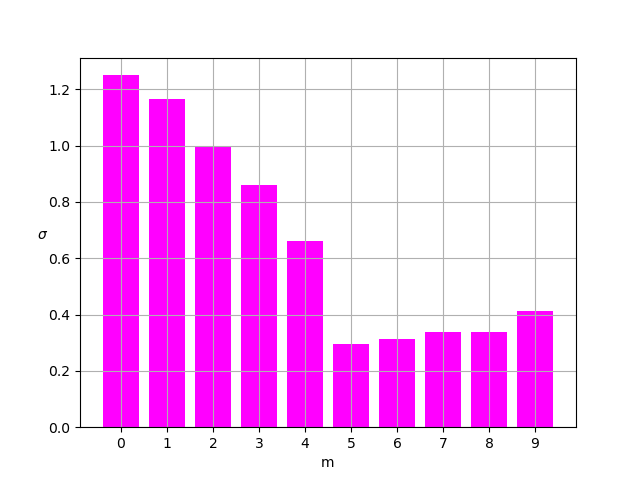
\includegraphics[width=\textwidth]{task1_hist.png}
    \caption{Гистограмма $\sigma_m$}
\end{subfigure}
\hfill
\begin{subfigure}{0.49\textwidth}
    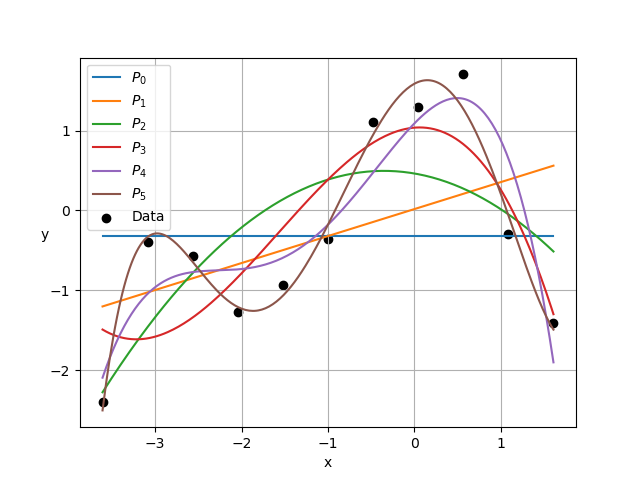
\includegraphics[width=\textwidth]{task1_polynoms.png}
    \caption{Графики многочленов $P_m(x)$}
\end{subfigure}

\caption{Результаты нахождения полиномов $P_m(x)$ по МНК.}
\end{figure}

По гистрограмме видно, что начиная с $m = 5$ значение $\sigma_m$ возрастает, соответственно $m^*=5$. Из графиков полиномов видно, что $P_5(x)$ лучше всего приближает имеющийся набор данных.



\newpage
\section{Задача 6.4.2. Траектория материальной точки}
\subsection{Формулировка задачи}
В таблице приведены результаты наблюдений за движением материальной точки в плоскости $(x, y)$. Известно, что движение осуществляется по кривой, описываемой многочленом $y = ax^m + b$. 

Используя МНК, необходимо определить коэффициенты $a$ и $b$, а также определить значение $\hat{x}$ координаты $x$, которое соответствует значению $\hat{y}$ координаты $y$. 

В соответствии с вариантом $m=2$ $\hat{y} = 8$, а таблица значений имеет следующий вид:
\begin{table}[h]
\centering
\hspace{0.1cm}
\begin{tabular}{|c|c|c|c|c|c|c|c|}
\hline
$x_i$ & 1.5 & 2.1 & 2.7 & 3.3 & 3.9 & 4.5 & 5.1  \\
\hline
$y_i$ & 11.1 & 10.3 & 9.08 & 7.64 & 5.92 & 3.9 & 1.6 \\
\hline
\end{tabular}
\end{table}

\subsection{Теоретический материал}
Для того, чтобы найти коэффициенты $a$, $b$ по методу наименьших квадратов необходимо решить систему линейных алгебраических уравнений:
\[
\begin{pmatrix}
    n & \sum\limits_{i=1}^n x_i^m \\
    \sum\limits_{i=1}^n x_i^m & \sum\limits_{i=1}^n x_i^{2m}
\end{pmatrix} \cdot \begin{pmatrix}
    b \\
    a
\end{pmatrix} = \begin{pmatrix}
    \sum\limits_{i=1}^n y_i \\
    \sum\limits_{i=1}^n y_i x_i^m
\end{pmatrix} 
\]

\subsection{Результаты}
\begin{table}[!h]
\centering
\begin{tabular}{|c|c|c|}
     \hline
     $b$ & $a$ & $\hat{x}$ \\
     \hline
     12.0205 & -0.4009 & 3.1667 \\
     \hline
\end{tabular}
\caption{Значения коэффициентов $b$ и $a$, найденные при помощи метода наименьших квадратов и величина $\hat{x}.$ }
\end{table}

\newpage
\begin{figure}[h]
    \centering
    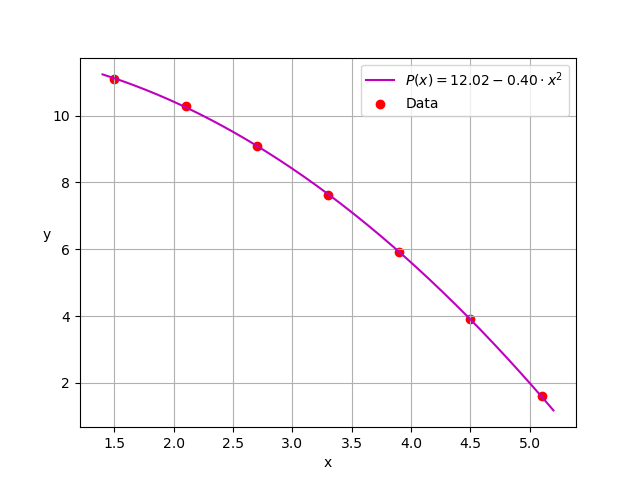
\includegraphics[width=\textwidth]{task2-polynomial.png}
    \caption{График функции $P(x) = b + ax^2$, где коэффициенты $a$ и $b$, были найдены при помощи метода наименьших квадратов.}
\end{figure}



\newpage
\section{Задача 6.7.5. Сравнение кусочно-линейной и глобальной интерполяции}
\subsection{Формулировка задачи}
Дана кусочно-гладкая функция $y=f(x)$. Необходимо сравнить приближения функции кусочно-линейной и глобальной интерполяциями.

Решение должно состоять из следующих шагов:
\begin{enumerate}
    \item Вычислить значения функции $f(x)$ в произвольных точках $x_i$, $i=0, \dots, k-1$ отрезка $[a, b]$, по которым будет осуществляться интерполяция.
    \item Реализовать программу, вычисляющую значение интерполяционного многочлена 1-ой степени по точкам $(x_i, y_i)$ и $(x_{i+1}, y_{i+1})$ в произвольной точке отрезка $[x_i, x_{i+1}]$. С её помощью вычислить приближённые значения $f(x)$ в $3k$ точках отрезка $[a, b]$.
    \item Написать программу, возвращающую значение интерполяционного многочлена в форме Ньютона (с разделёнными разностями). Вычислить приближённые значения $f(x)$ в тех же $3k$ точках.
    \item На одном чертеже построить графики интерполирующих функций, график $f(x)$, а также отметить точки, по которым осуществлялась интерполяция.
    \item Вычислить практическую величину погрешностей $\Delta_j$, $j = 0, \dots, 3k - 1$, приближения $f(x)$ в $3k$ точках для кусочно-линейной и глобальной интерполяций. На одном чертеже построить графики погрешностей.
\end{enumerate}

В соответствии с вариантом:
\[
f(x)=|x-1|e^x\ \ \ \ \ [a, b] = [0, 2]
\]


\subsection{Теоретический материал}
\subsubsection{Кусочно-линейная интерполяция}
Кусочно-линейная интерполяция - метод интерполяции, основная идея которого состоит в том, чтобы на отрезке $[x_{i-1}, x_i]$ приближать исходную функцию линейной функцией $f_i(x) = k_i x + b$, проходящей через точки $(x_{i-1}, y_{i-1})$ и $(x_i, y_i)$, то есть $f(x_{i-1}) = y_{i-1}, f(x_i) = y_i$.

Используя свойство выше можно выписать $f_i(x)$ в явном виде:
\[
f_i(x) = f(x_{i-1}) + \frac{f(x_i) - f(x_{i-1})}{x_i - x_{i-1}}
\left( x - x_{i-1} \right)
\]

\subsubsection{Интерполяционные формулы Ньютона}
В общем случае интерполяционный многочлен Ньютона - это многочлен, которые имеет вид:
\[
P_n(x) = f[x_0] + (x - x_0)f[x_0; x_1] + 
\dots + (x - x_0)(x - x_1)\dots(x - x_{n-1})f[x_0;\dots;x_n] 
\]
где $f[x_0;x_1;\dots;x_n]$ - разделённая разность порядка $n$.

Разделённая разность порядка $k$ определяется через разделённые разности порядка $k - 1$:

\[
f[x_0; x_1; \dots; x_k] = 
\frac{f[x_1; \dots; x_k] - f[x_0; \dots x_{k-1}]}{x_k - x_0}
\]
И в частности:
\[
f[x_0; x_1] = \frac{f(x_1) - f(x_0)}{x_1 - x_0} = 
\frac{y_1 - y_0}{x_1 - x_0}
\]

При этом разделённая разность может быть найдена с помощью следующей формулы:

\[
f[x_0; x_1; \dots; x_k] = \sum\limits_{i = 0}^{n}
\frac{f(x_i)}{
\prod\limits_{\substack{j = 0 \\ j \ne i}}^n(x_i - x_j)
}
\]
\newpage
\subsection{Код на Python}
\begin{minted}[
frame=single,
framesep=10pt,
framerule=0.1pt,
bgcolor=LightGray
]{python}
class LinearInterp1d:
    """
    Класс для линейной интерполяции.
    """
    def __init__(self, x, y):
        assert x.ndim == 1
        assert y.ndim == 1
        assert x.shape == y.shape
        
        self.a = x.min()
        self.b = x.max()
        self.segments = {}

        for i in range(1, x.size):
            x0, x1 = x[i-1], x[i]
            y0, y1 = y[i-1], y[i]
            
            k = (y1 - y0)/ (x1 - x0)
            b = 0.5 * (y0 + y1) - k / 2 * (x0 + x1)

            self.segments[(x0, x1)] = (k, b)

    def __call__(self, x):
        """
        Вычисляет значения функции в точках.
        """
        assert x.ndim == 1
        
        y = np.zeros(x.size)
        for i, x_p in enumerate(x):
            y[i] = self._interp1point(x_p)

        return y

    def _interp1point(self, x_p):
        """
        Вспомогательный метод для нахождения 
        значения функции в точке.
        """
        if x_p < self.a or self.b < x_p:
            raise ValueError(f'x={x_p}')

        kx, bx = None, None
        for (x0, x1), (k, b) in self.segments.items():
            if x0 <= x_p and x_p <= x1:
                kx = k
                bx = b
                break
        return k * x_p + b
\end{minted}

\begin{minted}[
frame=single,
framesep=10pt,
framerule=0.1pt,
bgcolor=LightGray
]{python}
class NewtonInterp1d:
    """
    Класс для интерполяции с помошью интеполяционного 
    многочлена в форме Ньютона.
    """
    def __init__(self, x, y):
        assert x.ndim == 1
        assert y.ndim == 1
        assert x.shape == y.shape

        n = x.size - 1
        self.n = n
        self.f_coeffs = np.zeros(n + 1)
        self.x_data = x.copy()

        for k in range(n + 1):
            divided_diff = 0.0
            for i in range(k + 1):
                divider = 1
                for j in range(k + 1):
                    if j == i:
                        continue
                    divider *= \ 
                    (self.x_data[i] - self.x_data[j])
                divided_diff += (y[i] / divider)
            self.f_coeffs[k] = divided_diff 
    
    def __call__(self, x):
        """
        Находит значения многочлена в точках. 
        """
        assert x.ndim == 1

        poly_res = 0.0
        term = 1
        for k in range(self.n + 1):
            poly_res += term * self.f_coeffs[k]
            term *= (x - self.x_data[k])
        return poly_res
\end{minted}

\newpage
\subsection{Результаты}
\begin{figure}[!h]
\centering
\begin{subfigure}{0.49\textwidth}
    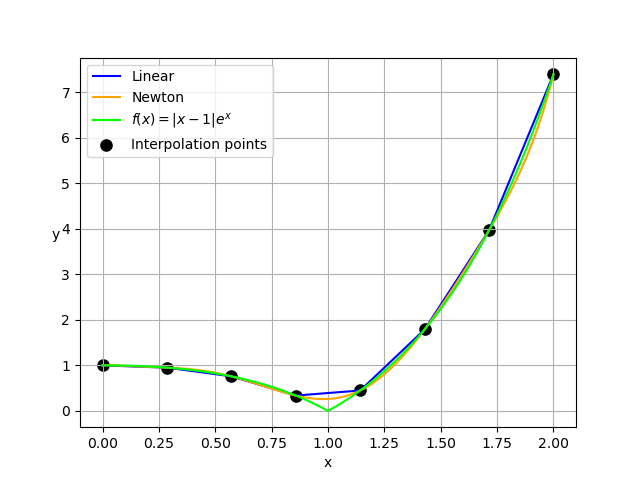
\includegraphics[width=\textwidth]{task3_intepolations.png}
    \caption{График $f(x)$ и интерполяций}
\end{subfigure}
\hfill
\begin{subfigure}{0.49\textwidth}
    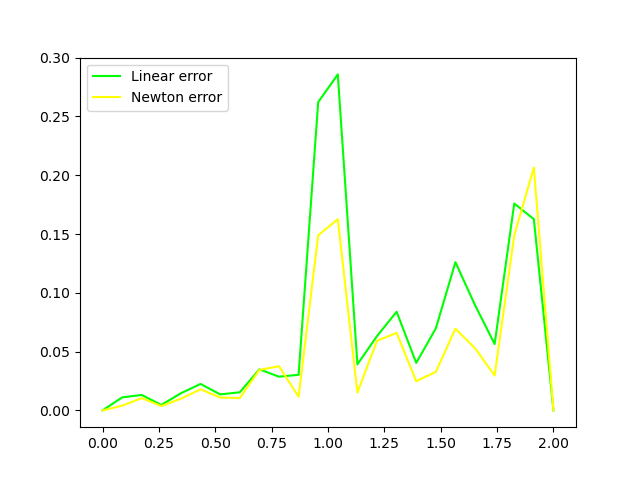
\includegraphics[width=\textwidth]{task3_errors.png}
    \caption{График ошибок интерполяций}
\end{subfigure}

\caption{Сравнение кусочно-линейной и глобальной интерполяций. Интерполяция производилась по $k=8$ точкам отрезка.}
\end{figure}

Видно, что кусочно-линейная интерполяция больше ошибается в окрестности точки $x = 1$. При этом на всём отрезке, за исключением небольшой окрестности точки $x=1$, обе интерполяции показывают примерно одинаковые ошибки. 



\newpage 
\section{Задача 6.9.5. Сплайн-интерполяция}
\subsection{Формулировка задачи}
Дана функция $y=f(x)$. Необходимо приблизить $f(x)$ на отрезке $[a, b]$ методом глобальной интерполяции и указанным в варианте сплайном. На одном чертеже построить графики приближающей функции и $f(x)$. Сравнить качество приближения при разном количестве узлов интерполяции. 

Согласно условию варианта, сплайн - кубический дефекта 1, $f(x)=\frac{\cos(x^3)}{x}$, $a = 1,\ b = 2.75$.
\subsection{Теоретический материал}
Пусть функция $f(x)$ задана на отрезке $[a, b]$, разбитом на части $[x_{i-1}, x_i]$, $a = x_0 < x_1 < \dots < x_n = b$. Кубическим сплайном дефекта 1 называется функция $S(x)$, которая:
\begin{itemize}
    \item на каждом отрезке $[x_{i-1}, x_i]$ является многочленом степени не выше третьей.
    \item имеет непрерывные первую и вторую производные на $[a, b]$.
    \item в точках $x_i$ выполняется равенство $S(x_i) = f(x_i)$, то есть сплайн $S(x)$ интерполирует функцию $f(x)$ в точках $x_i$.
\end{itemize}
Для однозначного задания сплайна перечисленных выше условий недостаточно, необходимо наложить граничные условия. Одним из вариантов таких условий, который мы будем дальше использовать, является \textit{естественный сплайн} - граничные условия вида $S''(a) = S''(b) = 0$. 

Пусть на отрезке $[x_{i-1}; x_i]$ выражается как 
\[
S(x) = S_i(x) = a_i + b_i (x - x_i) + c_i (x - x_i)^2 + d_i (x - x_i)^3
\]
тогда для \textit{естественного сплайна} можно выписать формулы для нахождения $a_i$, $b_i$, $c_i$, $d_i$:
\[
a_i = f(x_i)
\]
\[
d_i = \frac{c_i - c_{i-1}}{3h_i}
\]
\[
b_i = \frac{a_i - a_{i-1}}{h_i} - 
\frac{2 \cdot c_{i-1} + c_i}{3} \cdot h_i
\]
\[
c_{i-1}\cdot h_i + 2c_i \cdot (h_i + h_{i+1}) + c_{i+1}\cdot h_{i+1} = 
3 \cdot \left(
\frac{a_{i + 1} - a_i}{h_{i + 1}} - \frac{a_i - a_{i-1}}{h_i}
\right)
\]
где $h_i = x_i - x_{i-1}$, и при этом $c_n = S''(x_n)=0$, $c_1 - 3 d_1 h_1 = S''(x_0) = 0$.

\newpage
\subsection{Результаты}
\begin{figure}[!h]
\centering
\begin{subfigure}{0.99\textwidth}
    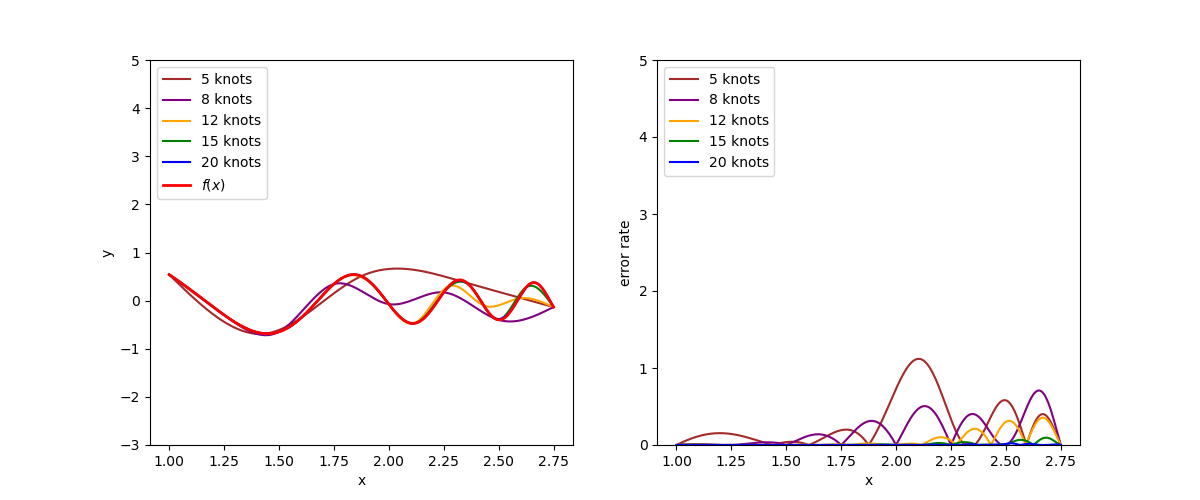
\includegraphics[width=\textwidth]{task4_cubic-interp.png}
    \caption{Кубический сплайн дефекта 1}
\end{subfigure}
\hfill
\begin{subfigure}{0.99\textwidth}
    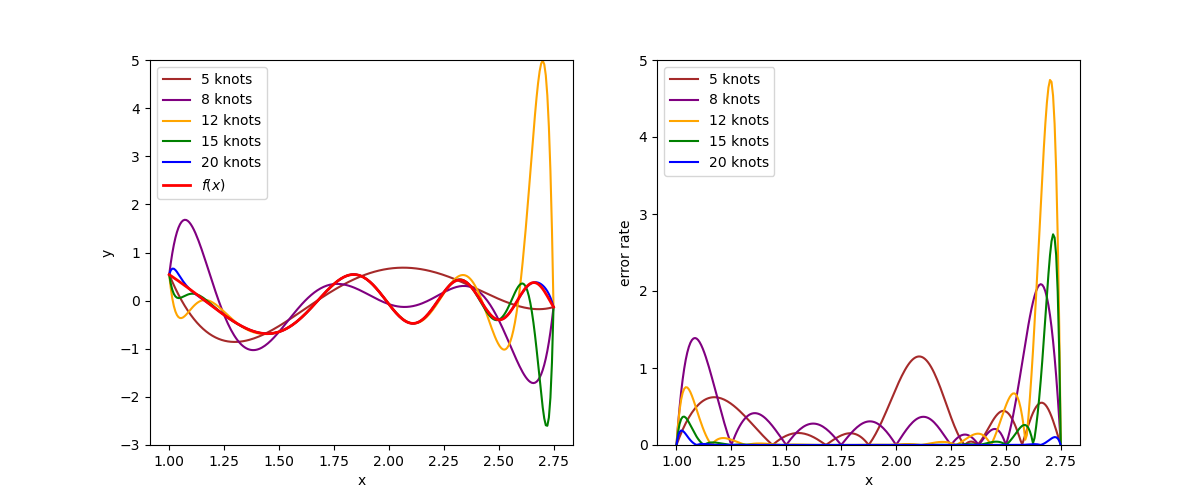
\includegraphics[width=\textwidth]{task4_global-interp.png}
    \caption{Глобальная интерполяция по формулам Ньютона}
\end{subfigure}

\caption{Интерполяция функции $f(x)$ при разном количестве узлов интерполяции. На левых рисунках изображены интерполяции и $f(x)$, на правых - ошибки интерполяций.}
\end{figure}

Видно, кубический сплайн лучше приближает $f(x)$, нежели интерполяционный многочлен Ньютона. При этом для кубического сплайна, уже начиная с 15 узлов визуально очень трудно отличить $f(x)$ от интерполяции.

\end{document}